\documentclass{article}
\usepackage[utf8]{inputenc}
\usepackage[portuguese]{babel}
\usepackage{subcaption}
\usepackage{amsmath}
\usepackage{amssymb}
\usepackage{graphicx}
\usepackage{listings}
\usepackage{hyperref}
\usepackage{float}
\usepackage{lstdoc}


\begin{document}

    \begin{center}
        \Large \textbf{Universidade Estadual de Campinas} \\
        \large Instituto de Computação \\
        \vspace{0.5cm}
        \large Introdução ao Processamento Digital de Imagens (MC920 / MO443) \\
        \large Professor: Hélio Pedrini
    \end{center}

    \vspace{2cm}

    \begin{center}
        \LARGE \textbf{Trabalho 4} \\
        \vspace{0.5cm}
        \Large Julio Vinicius Amaral Oliveira – 230537
    \end{center}

    \vspace{2cm}

    \begin{flushright}
        \large \textbf{Data de Entrega:} 13 de junho de 2025
    \end{flushright}

    \newpage


    \section{Introdução}\label{sec:introducao}
    O objetivo deste relatório é aplicar 2 algoritmos, o primeiro que deve identificar os contornos dos objetos de uma imagem, além de suas características como:
    área, perímetro, excentricidade e solidez.
    O segundo, deve ser capaz de realizar tanto a rotação quando ampliação de uma imagem, utilizando interpolações para tal.
    As interpolações que vamos trabalhar são: Lagrange, bicúbica, bilinear e pelo vizinho mais próximo.


    \section{Especificação do Problema}\label{sec:especificacao-do-problema}
    O objetivo principal é desenvolver um programa que: consiga realizar a identificação de do contorno dos objetos além
    de mostrar suas propriedades e também desenvolver outro que: consiga, utilizando interpolação, realizar a rotação e
    redimensionamento de imagens.


    \section{Detecção de contornos}\label{sec:deteccao-de-contornos}

    \subsection{Bibliotecas utilizadas}\label{subsec:bibliotecas-utilizadas}
    Para realização do objetivo, utilizamos algumas bibliotecas como \texttt{argparse} para criação das flags,
    \texttt{cv2} para leitura e algumas operações com imagens, \texttt{skimage} para obter os ids de cada imagem, propriedades, etc,
    \texttt{numpy} para realizarmos operações matemáticas e por fim o \texttt{matplotlib} para gerar os histogramas solicitados

    \subsection{Descrição do programa}\label{subsec:descricao-do-programa}
    Primeiramente, realizamos a leitura e conversão das imagens usando o \texttt{open-cv}, após isso com a ajuda do
    \texttt{threshold\_otsu} obtemos o valor de threshold e também criamos os labels das regiões.
    Depois, obtemos as propriedades de cada região com o auxílio da classe \texttt{measure} do \texttt{skimage} e para
    cada propriedade imprimimos nos arquivos de output seus valores.
    O próximo passo, foi detectar os contornos da imagem com a ajuda do \texttt{open-cv}, após acharmos seus contornos
    com a função \texttt{cv2.findContours} os desenhamos em um fundo branco com \texttt{cv2.drawContours} em vermelho.
    Após isso, a próxima tarefa foi mostrar os objetos com seus respectivos ids, para isso, bastou utilizar o método
    \texttt{color.label2rgb} do \texttt{skimage} e depois precisamos somente escrever os respectivos números acima de cada objetos,
    para isso achamos o centro e deslocamos ele em x e y considerando o tamanho do texto de forma que esse ficasse no centro
    do seu respectivo objeto.
    Por fim, tivemos apenas que percorrer cada objeto e os classificar como pequeno médio ou grande utilizando um laço de repetição simples.
    Também plotamos o histograma das áreas utilizando funcionalidades simples da biblioteca \texttt{matplotlib}.


    \section{Transformações geométricas}\label{sec:transformacoes-geometricas}

    \subsection{Bibliotecas utilizadas}\label{subsec:bibliotecas-transformacao}
    Para implementar rotação e redimensionamento de imagens, utilizamos algumas bibliotecas como
    \texttt{argparse} para criação das flags, \texttt{cv2} para operações com imagens como leitura, escrita, etc e
    \texttt{numpy} para as operações com matrizes e interpolação.

    \subsection{Descrição do programa}\label{subsec:descricao-transformacao}
    Primeiramente, realizamos a leitura e conversão das imagens usando o \texttt{open-cv}.
    Depois, criamos quatro rotinas de interpolação que podem ser escolhidas pelo usuário no momento da inicialização do código:
    vizinho mais próximo, bilinear, bicúbica e Lagrange.
    Cada uma delas recebe coordenadas \((x',y')\) da imagem original e devolve o valor interpolado utilizando o respectivo método escolhido:

    \begin{itemize}
        \item \textbf{Vizinho mais próximo:} simplesmente arredonda \((x',y')\) para o pixel inteiro mais próximo.
        \item \textbf{Bilinear:} calcula a média ponderada dos quatro pixels vizinhos que formam o quadrado ao redor de \((x',y')\).
        \item \textbf{Bicúbica:} utiliza a função B-spline para realizar a interpolação
        \item \textbf{Lagrange:} aplica polinômios de Lagrange.
    \end{itemize}

    Encapsulamos todas as funções numa função \texttt{interpolate}, que recebe a imagem, as coordenadas e o método desejado.
    Essa função então escolhe qual interpolação aplicar com base no que o usuário escolheu.
    Optamos por não detalhar a fundo as funções, já que sua implementação é apenas a codificação das funções apresentadas no comando do trabalho.


    \section{Principais desafios}\label{sec:principais-desafios}

    \subsection{Detecção de contornos}\label{subsec:desafios-deteccao-de-contornos}
    Os métodos criados para resolução do problema não foram muito desafiadores, se tratando mais de aplicação simples de métodos
    já existentes em bibliotecas open source.
    Porém, considerei desafiador a pesquisa para encontrar os métodos que conseguissem resolver os problemas propostos.

    \subsection{Transformações geométricas}\label{subsec:desafios-transformacoes-geometricas}
    O desafio apresentado envolvia basicamente a implementação das fórmulas apresentadas no enunciado, algumas sendo relativamente
    simples de implementar como a de vizinhos próximos outras que apresentaram uma complexidade alta.
    Como a de lagrange, que demandou bastante refatorações até chegar em um código limpo.
    Também foi um desafio lidar com as bordas, que durante o desenvolvimento causaram bastantes bugs ao longo do código e que
    exigiram um manuseio cuidadoso ao longo do código.


    \section{Resultados}\label{sec:resultados}
    Os resultados obtidos para os respectivos desafios foram

    \subsection{Detecção de contornos}\label{subsec:resultados-deteccao-de-contornos}
    Para o objeto 2, que possuia mais objetos:
    \begin{figure}[H]
        \centering
        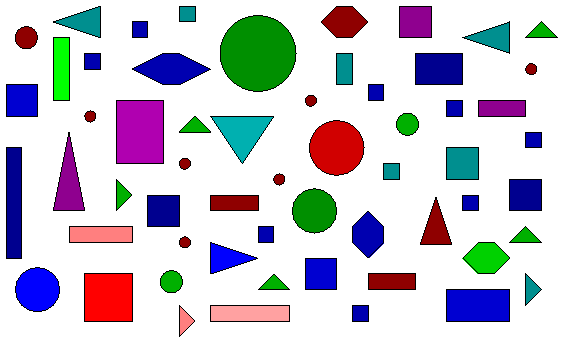
\includegraphics[width=0.6\textwidth]{../input/objetos2}
        \caption{Objeto 2 com diferentes formados}
    \end{figure}
    Conseguimos obter seus contornos e seus rótulos:

    \begin{figure}[H]
        \centering
        \begin{subfigure}{0.45\textwidth}
            \centering
            
\includegraphics[width=\textwidth]{../output/parte01/contornos}
            \caption{Contornos da imagem}
            \label{fig:contornos-objeto-2}
        \end{subfigure}
        \hfill
        \begin{subfigure}{0.45\textwidth}
            \centering
            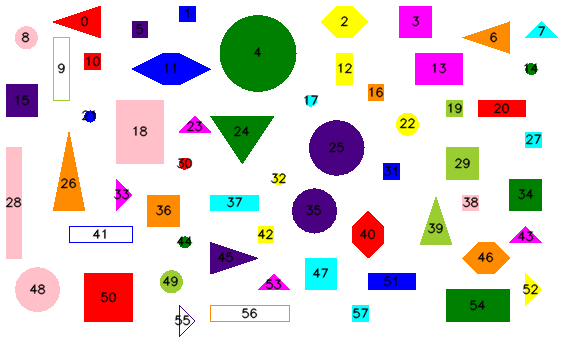
\includegraphics[width=\textwidth]{../output/parte01/regioes_rotuladas}
            \caption{Rótulos da imagem}
            \label{fig:imagem2}
        \end{subfigure}
        \caption{Resultados obtidos}
    \end{figure}
    Além de seu histograma:
    \begin{figure}[H]
        \centering
        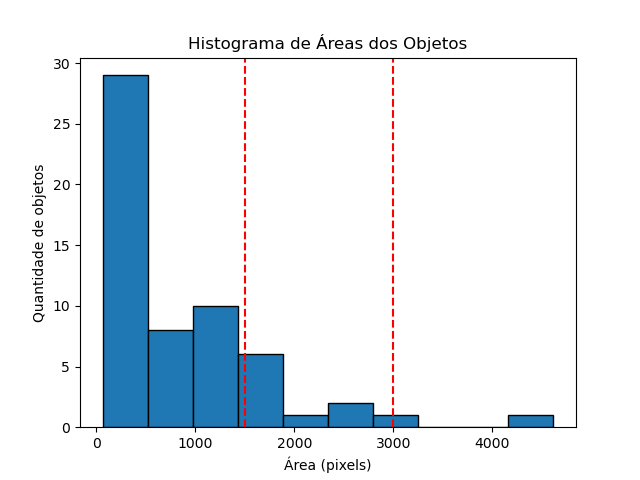
\includegraphics[width=0.8\textwidth]{../output/parte01/histograma_areas}
        \caption{Histograma de áreas}
    \end{figure}

    \subsection{Transformação}\label{subsec:resultados-transformacao}
    Utilizamos o objeto 1 para os testes:
    \begin{figure}[H]
        \centering
        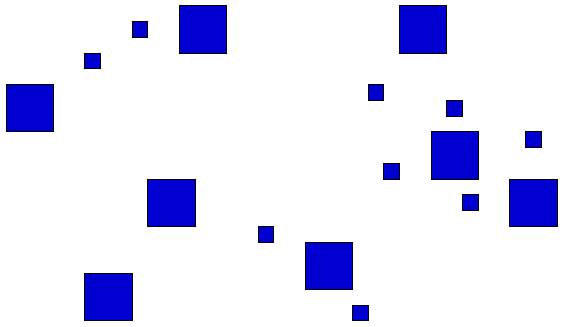
\includegraphics[width=0.6\textwidth]{../input/objetos1}
        \caption{Objeto 1}
    \end{figure}
    Seguem alguns resultados

    \begin{figure}[H]
        \centering
        
\includegraphics[width=0.6\textwidth]{../output/parte02/objetos1_rotate_45deg_bicubic}
        \caption{Objeto 1 rotacionado em 45 graus (bicúbica)}
    \end{figure}

    \begin{figure}[H]
        \centering
        \begin{subfigure}{0.45\textwidth}
            \centering
            
\includegraphics[width=\textwidth]{../output/parte02/objetos1_scale_2.00x2.00_bicubic}
            \caption{Bicúbica redimensionada para 2x2}
            \label{fig:objeto1-redimensionado-bicubic}
        \end{subfigure}
        \hfill
        \begin{subfigure}{0.45\textwidth}
            \centering
            
\includegraphics[width=\textwidth]{../output/parte02/objetos1_scale_2.00x2.00_bilinear}
            \caption{Bilinear redimensionada para 2x2}
            \label{fig:objeto1-redimensionado-bilinear}
        \end{subfigure}
        \caption{Interpolações Bicúbica e Bilinear}
    \end{figure}

    \begin{figure}[H]
        \centering
        \begin{subfigure}{0.45\textwidth}
            \centering
            
\includegraphics[width=\textwidth]{../output/parte02/objetos1_scale_2.00x2.00_lagrange}
            \caption{Lagrange redimensionada para 2x2}
            \label{fig:objeto1-redimensionado-lagrange}
        \end{subfigure}
        \hfill
        \begin{subfigure}{0.45\textwidth}
            \centering
            
\includegraphics[width=\textwidth]{../output/parte02/objetos1_scale_2.00x2.00_nearest}
            \caption{Nearest redimensionada para 2x2}
            \label{fig:objeto1-redimensionado-nearest}
        \end{subfigure}
        \caption{Interpolações Lagrange e Nearest Neighbor}
    \end{figure}


    \section{Conclusão}\label{sec:conclusao}
    As implementações dos algoritmos para resolução dos problemas propostos foram bem eficazes, e conforme os resultados
    mostraram, eles conseguiram atender às solicitações.
    Como ponto de melhorias, podemos melhorar o desempenho das transformações que utilizam lagrange, pois notamos que o
    tempo de execução era bem grande para algumas imagens.
    Além disso, as imagens que foram rotacionadas, foram cortadas preservando as medidas de largura e altura originais,
    uma melhoria que poderia ser feita é melhorar isso de forma que a imagem rotacionada não tivesse mais esse corte.

\end{document}